\chapter{Introduction}
% \section*{19 - Settembre}
\subsection*{Info and Contact}
% Ricevimento Lunedì 14:30 - 16:00/16:30

\href{https://pages.di.unipi.it/corradini/Didattica/AP-23/}{Pagina del corso}
% \href{http://didawiki.di.unipi.it/doku.php/magistraleinformaticanetworking/ae/ae2023/start}{Didawiki Corso}
\section{Introduction}
\subsection{Framework}
A software \textbf{framework} is a collection of common code providing generic functionality that can selectively overridden or specialized by user code providing specific functionality.

When using \textit{frameworks} there is an \textbf{inversion of control}.
Differently from what happens when using libraries,
the program-flow is dictated by the framework, not by the caller.

\subsection{Design Patterns}
A \textbf{design pattern} is a general reusable solution to a commonly occurring problem within a given context in software design. 
A design pattern is characterized by:
\begin{itemize}
    \item \textbf{Name}
	\item \textbf{Problem Addressed}
	\item \textbf{Context} - Used to determine applicability
	\item \textbf{Forces} - Constraints or issues that the solution must address
	\item \textbf{Solution} - It must resolve all \textit{forces}
\end{itemize}

% \section*{20 - Settembre}
% Goldbolt is a useful tool, to see preprocessor output, compiling, ecc.
\subsection{Programming Languages}
A \textbf{PL} is defined via \textbf{syntax}, \textbf{semantics} and \textbf{pragmatics}\footnote{the way in which the PL is intended to be used in practice}.
\subsubsection{Syntax}
Used by the compiler for \textit{scanning} and \textit{parsing}.
The \textit{lexical} grammar defines the syntax of token (e.g. "for" blocks, constants)
\subsubsection{Semantics}
Semantics might be described using natural language, which even if precise, allows ambiguousity.
\textbf{Formal} approches to semantics definition are:
\begin{enumerate}
    \item \textit{Denotational} - Mapping every syntactic entity with a mathematical entity
    \item \textit{Operational} - Defining a computation relation in a form $e \Rightarrow v$, where $e$ is a program
    \item \textit{Axiomatic} - Based on Hoare-triples $\textit{Precondition} \wedge \textit{Program}\Rightarrow \textit{Postcondition}$ 
\end{enumerate}
However, they rarely scale to fully-fledged programming languages.
\subsubsection{Pragmatics}
\textit{Pragmatics} include coding conventions, guidelines for elegant code, etc.

\subsection{Programming Paradigms}
Paradigms belong to languages \textit{pragmatics}, not to the way the language is defined, i.e. not syntax nor semantics.
\begin{enumerate}
    \item \textbf{Imperative}
    \item \textbf{Object-oriented}
    \item \textbf{Concurrent} - Processes, communication, \dots 
    \item \textbf{Functional} - values, expressions,
    functions, higher-order functions, \dots
    \item \textbf{Logic} - Assertions, relations, \textit{strange sorceries}\dots 
\end{enumerate}

Modern PLs, provide constructs and solutions to program in all these paradigms

\subsection{Implementing PLs}
\begin{itemize}
    \item Programs written in \textbf{L} must be \textit{executable}
    \item Every language \textbf{L} implicitly defines and \textit{Abstract Machine} \textbf{$M_L$} having \textbf{L} as a Machine Language
    \item Implementing $M_L$ on an existing host machine $M_O$ via compilation or interpretation (or both) makes programs written in \textbf{L} executables 
\end{itemize}

An \textbf{Abstract Machine} $M_L$ for $L$ is a \ul{collection of data structures and algorithms which can perform the storage and execution of programs written in L.}\\
Viceversa, $M$ defines a language $L_M$ including all programs which can be executed by the interpreter $M$.\\
There is a \ul{bidirectional correspondance} between machines and languages components.\\
\begin{center}
$
\begin{array}{ccc}
    \textit{Primitive data processing} & \longleftrightarrow & \textit{Primitive data types}  \\
    \textit{Sequence control} & \longleftrightarrow & \textit{Control structures}  \\
    \textit{Data transfer control }& \longleftrightarrow & \textit{Parameter passing and value return}  \\
    \textit{Memory management }& \longleftrightarrow & \textit{Memory management}\\
     & 
\end{array}
$   
\end{center}

\begin{center}
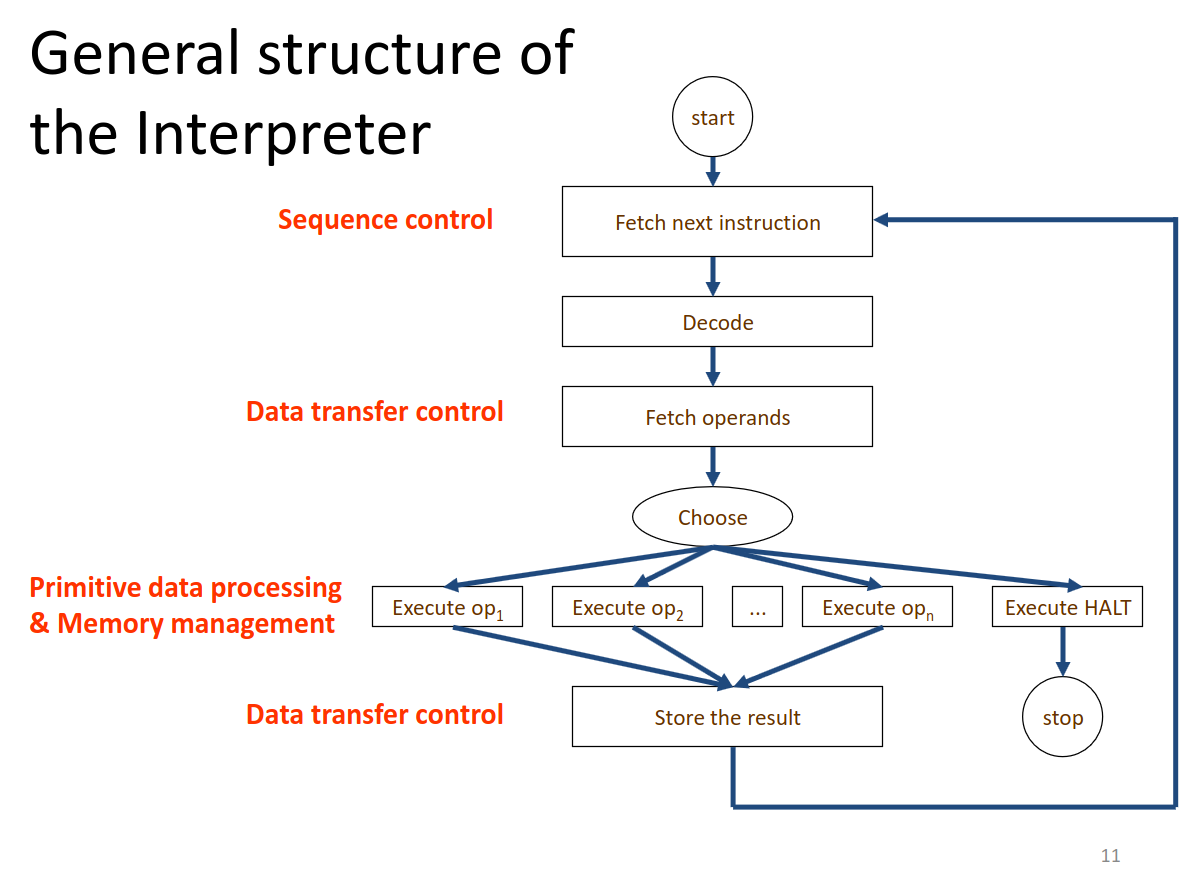
\includegraphics[width=0.7\textwidth]{images/interpreter_structure.png}
\end{center}

In computer science one of the main focuses is \textbf{abstraction}, and this applies also to the implementation of AMs, leading to an onion-like structure, or \textbf{hierarchical} structure,
as can be seen in the scheme in \ref{fig:machines_hierarchy}.

\begin{figure}[htbp]
    \centering
    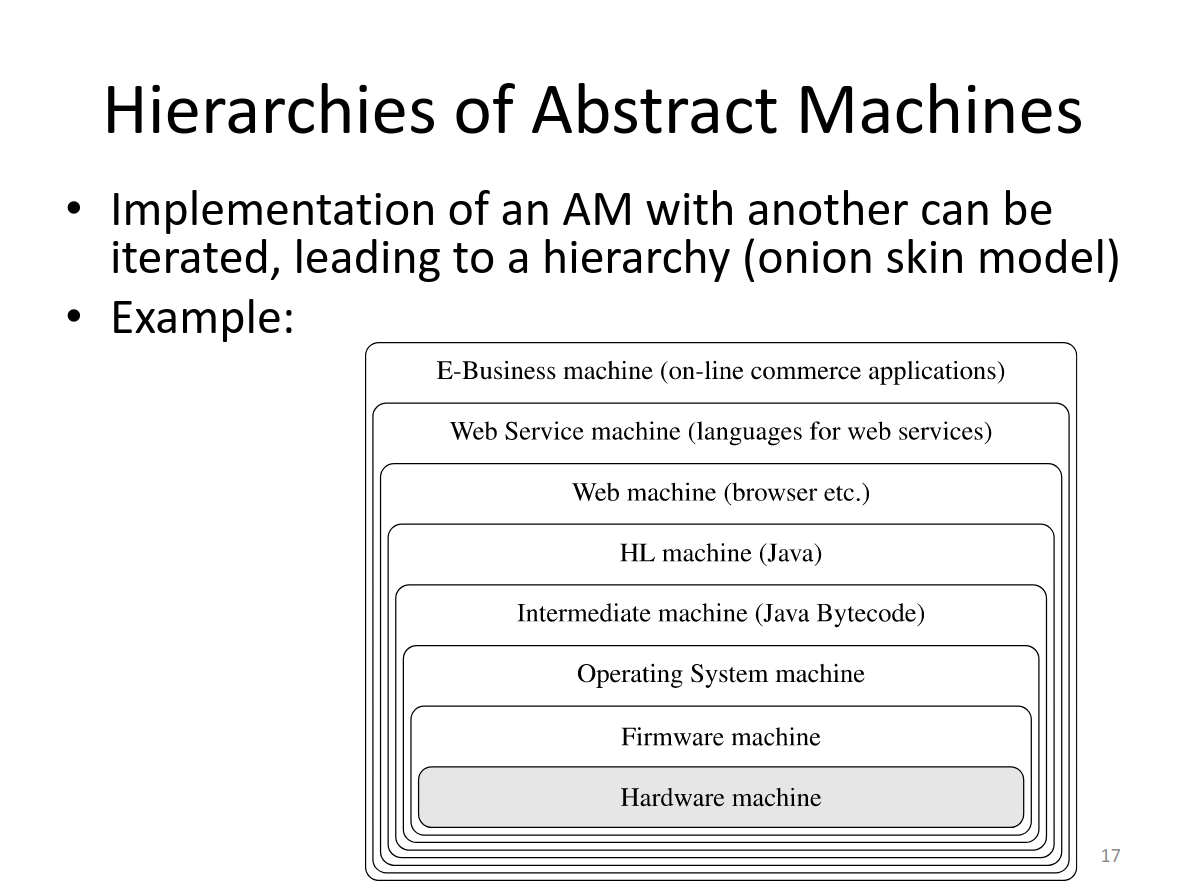
\includegraphics{images/machines_hierarchy.png}
    \caption{AM Hierarchical Structure}
    \label{fig:machines_hierarchy}
\end{figure}

% A software component is a unit of composition with
% contractually specified interfaces and explicit context
% dependencies only. A software component can be
% deployed independently and is subject to
% composition by third parties.

\subsection*{Implementing PLs - Wrap Up}
\begin{itemize}
    \item $L$ High-level programming language
    \item $M_L$ Abstract machine for $L$
    \item $M_O$ host machine
\end{itemize}

\subsubsection{Pure Interpretation}

\begin{figure}[htbp]
    \centering
    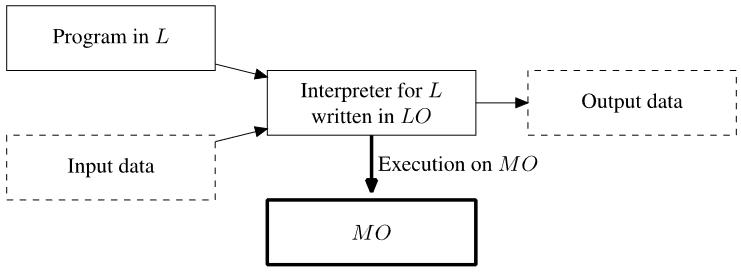
\includegraphics{images/am_pure_int.png}
    \caption{Pure Interpretation}
    \label{fig:am_pure_int.png}
\end{figure}

$M_L$ is interpreted over $M_O$.
It isn't very efficient, mainly because of fetch-decode phases

\subsubsection{Pure Compilation}

\begin{figure}[htbp]
    \centering
    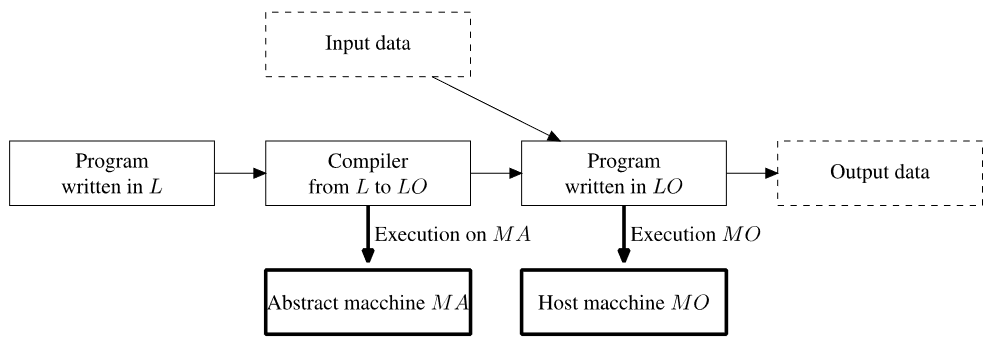
\includegraphics{images/am_pure_comp.png}
    \caption{Pure Compilation}
    \label{fig:am_pure_comp.png}
\end{figure}

$L$ programs are translated into $L_O$, the machine laguange of $M_O$,
hence, $M_L$ is not realized at all and the programs are directly executed on $M_O$.\\
\textit{Compilation} is more efficient than \textit{Interpretation}, 
but produced code is larger

\subsubsection{Both}

\begin{figure}[htbp]
    \centering
    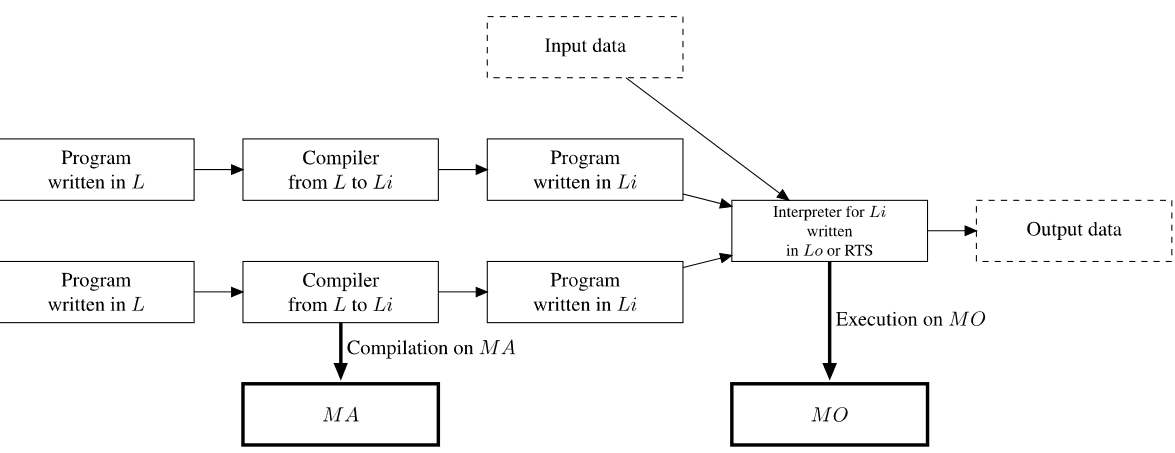
\includegraphics{images/am_both.png}
    \caption{Both}
    \label{fig:am_both}
\end{figure}

All real languages use both \textit{interpretation} and \textit{compilation}, the \textit{``pure''} cases are only limit cases.

Some languages, e.g. Java, use an intermediate Abstract Machine, called a \textit{Virtual Machine},
which increases \textit{Portability} and \textit{Interoperability}.

\begin{itemize}
	\item Compilation leads to better performance in general
	    \begin{itemize}
		    \item Allocation of variables without variable lookup at run time
		    \item Aggressive code optimization to exploit hardware features
	    \end{itemize}
	\item Interpretation facilitates interactive debugging and testing
	    \begin{itemize}
		    \item Interpretation leads to better diagnostics of a programming problem
		    \item Procedures can be invoked from command line by a user
		    \item Variable values can be inspected and modified by a user
	    \end{itemize}
\end{itemize}
